\documentclass[a4paper, 10pt]{book}

\usepackage{wrapfig}

\usepackage{graphicx}
\usepackage{float}

\usepackage{tikz}
\usepackage{amsmath}

\usepackage{fontspec} % --fontspec-- package to use other fonts
\setmainfont{Vazirmatn-Regular.ttf} 
\newfontfamily\bold{Vazirmatn-Bold.ttf}

\usepackage{hyperref}

\usepackage{color}

\usepackage{geometry}
\geometry{top=2cm, bottom=2cm, left=1.5cm, right=1.5cm}

\title{\huge {\bold Parallel Algorithms}}
\author{Professor\\{\bold Dr. Masoumeh Damroudi}}
\date{Author\\{\bold Mohammad Khorshidi}}

\linespread{1.3}

\begin{document}

    \pagenumbering{roman}
    \maketitle
    \newpage

    \begin{center}
        \Large {\bold Course Overview}
    \end{center}

    In this lecture note, I have documented my personal interpretations and understanding of the material. Please note that there may be inaccuracies, and it is recommended to consult primary and authoritative sources for complete and accurate information. Additionally, I welcome any contributions to improve and refine this note. If you are reading this and would like to offer suggestions, feel free to do so via pull requests on my \href{https://github.com/elprofesorsunny/Master/tree/main/Papers/Parallel%20Aalgorithms/Booklet}{\textcolor{blue}{\bold GitHub}} or by emailing me at \href{mailto:someone@somewhere.com}{\textcolor{blue}{\bold mohammad\_khorshidi@outlook.fr}}.

    \section{Course Structure}

    \section{Instructor's Approach}

    \section{Grading and Evaluation}

        The grading structure for this course is as follows, with students expected to earn their grades based on the criteria outlined below:

        \begin{itemize}
            
            \item {\bold Presentation:} 4 points will be awarded for presenting and explaining a paper related to one aspect of parallelization, accompanied by its relevant implementation.

            \item {\bold Midterm Exam:} 4 points will be given for the midterm exam.

            \item {\bold Final Exam:} 12 points will be awarded for the final exam.

        \end{itemize}

        Additionally, students are expected to attend all classes and give due attention to the assignments that will be provided throughout the semester.
        
    \section{Course Materials and Resources}

    \tableofcontents
    
    \chapter{{\bold Introduction}}

    \pagenumbering{arabic}

        In today’s world, with the increasing volume of data and the need for faster computations, parallel algorithms have emerged as an effective method to enhance the performance of computing systems. Parallel algorithms allow us to divide a problem into smaller sub-problems, each of which can be processed simultaneously by multiple processors. This not only speeds up processing but also optimizes the use of hardware resources.

        In this lecture note, we will explore fundamental concepts of parallel processing, computational models such as the PRAM model, and interconnection structures like network links. We will also delve into the principles of designing and analyzing parallel algorithms, covering key metrics such as performance, speedup, and scalability. Our goal is to provide a comprehensive understanding of the challenges and opportunities in the field of parallel algorithms.

        Parallel algorithms play a crucial role in improving the performance of complex and resource-intensive computations. The primary goal of parallel algorithms is to divide a large problem into smaller, independent sub-problems, which can be solved simultaneously by multiple processors. This technique is essential in multi-core and distributed computing environments such as supercomputers and large computing clusters.

        The need for parallel computation arises from the requirement to process large amounts of data or perform complex computations in a reasonable amount of time. A parallel computer, which consists of multiple processing units or processors, enables this by dividing a large problem into smaller sub-problems. Each of these sub-problems is solved independently and simultaneously by separate processors. The results are then combined to solve the original problem more efficiently.

        This approach, known as parallel computing, leverages the power of multiple processors to work on different parts of a problem at the same time. By doing so, it accelerates the overall computation and makes optimal use of hardware resources. Algorithms that are specifically designed to utilize parallel computing, called parallel algorithms, are key to solving complex problems faster and more efficiently by running them on parallel computer architectures.

        \section{Computational Models}

            In any computing system, whether sequential or parallel, the instructions are executed based on the flow of data. The execution flow dictates the sequence in which the tasks are carried out by the computer and what needs to be done at each stage of execution.

            The flow of data through the instructions influences how they operate. Understanding the correct computational model is crucial for designing parallel algorithms. These models determine the architecture and behavior of the system, impacting the performance and efficiency of parallel computation.

            Flynn, in 1966, introduced a taxonomy of computer architectures based on instruction and data streams. The four major classes of this classification are:

            \begin{itemize}
                
                \item {\bold SISD (Single Instruction, Single Data):} A single instruction is executed on a single data stream.
                
                \item {\bold MISD (Multiple Instruction, Single Data):} Multiple instructions are executed on a single data stream.

                \item {\bold SIMD (Single Instruction, Multiple Data):} A single instruction is executed on multiple data streams simultaneously.

                \item {\bold MIMD (Multiple Instruction, Multiple Data):} Multiple instructions are executed on multiple data streams simultaneously.

            \end{itemize}

            \begin{figure}[H]

                \centering
                
                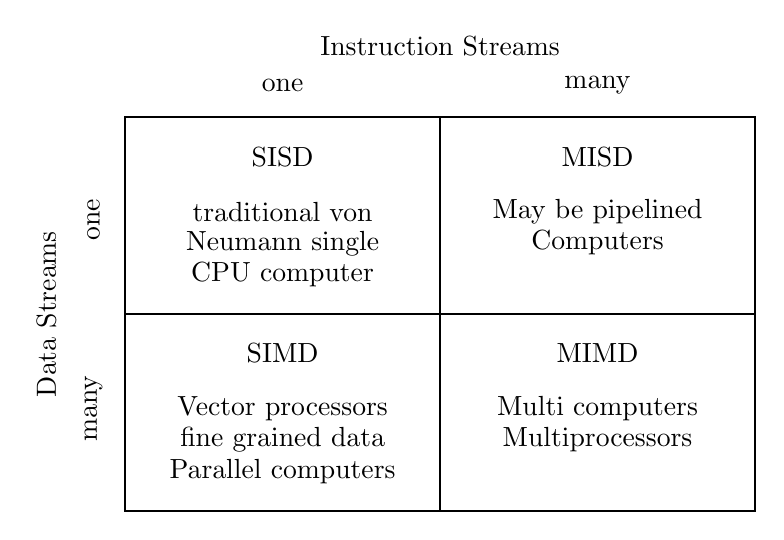
\begin{tikzpicture}
                    % Draw the grid lines
                    \draw[thick] (0,0) rectangle (8,5);
                    \draw[thick] (0,2.5) -- (8,2.5);
                    \draw[thick] (4,0) -- (4,5);
                    
                    % Add labels for SISD, SIMD, MISD, MIMD
                    \node at (2,4.5) {{\bold SISD}};
                    \node at (6,4.5) {{\bold MISD}};
                    \node at (2,2) {{\bold SIMD}};
                    \node at (6,2) {{\bold MIMD}};
                    
                    % Add descriptions for each category
                    \node at (2,3.8) {traditional von};
                    \node at (2,3.4) {Neumann single};
                    \node at (2,3) {CPU computer};
                    
                    \node at (6,3.8) {May be pipelined};
                    \node at (6,3.4) {Computers};
                    
                    \node at (2,1.3) {Vector processors};
                    \node at (2,0.9) {fine grained data};
                    \node at (2,0.5) {Parallel computers};
                    
                    \node at (6,1.3) {Multi computers};
                    \node at (6,0.9) {Multiprocessors};
                    
                    % Label axes
                    \node[rotate=90] at (-1,2.5) {Data Streams};
                    \node[rotate=90] at (-0.4,3.7) {one};
                    \node[rotate=90] at (-0.4,1.3) {many};
                    
                    \node at (2,5.4) {one};
                    \node at (6,5.4) {many};
                    \node at (4,5.9) {Instruction Streams};
                    
                \end{tikzpicture}
                
                \caption{A comparison between SISD, MISD, SIMD, and MIMD architectures}
            
            \end{figure}

            \subsection{SISD Architecture: Time Complexity and Characteristics}

            \begin{wrapfigure}{r}{0.5\textwidth}
                    
                \centering

                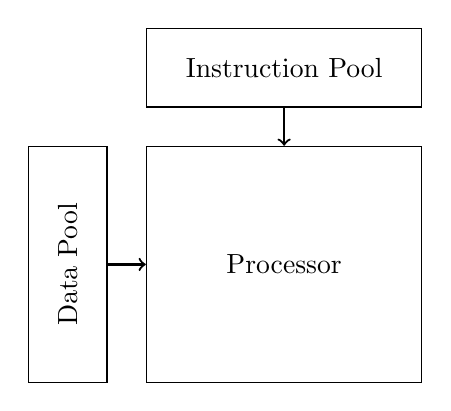
\begin{tikzpicture}
                    
                        % Data Pool
                        \node[draw, minimum width=3cm, minimum height=1cm, rotate=90]  (data) at (0.25,0) {Data Pool};
                        
                        % Instruction Pool
                        \node[draw, minimum width=3.5cm, minimum height=1cm] (instruction) at (3,2.5) {Instruction Pool};
                        
                        % Processor
                        \node[draw, minimum width=3.5cm, minimum height=3cm] (processor) at (3,0) {{\bold Processor}};
                        
                        % Arrows
                        \draw[thick, ->] (data.south) -- (processor.west);
                        \draw[thick, ->] (instruction.south) -- (processor.north);

                \end{tikzpicture}

                \caption{A conceptual diagram of SISD architecture.}

            \end{wrapfigure}

                The Single Instruction Single Data (SISD) architecture, introduced by John von Neumann in the late 1940s, processes one instruction at a time over a single data stream. This sequential nature means it doesn't support parallel processing, requiring only one processor to execute the tasks.

                An SISD computing system is a uniprocessor machine which is capable of executing a single instruction, operating on a single data stream. In SISD, machine instructions are processed in a sequential manner and computers adopting this model are popularly called sequential computers. Most conventional computers have SISD architecture. All the instructions and data to be processed have to be stored in primary memory.

                In the SISD model, the algorithm works in a serial fashion. For example, to sum a sequence of $n$ numbers, the algorithm accesses the memory $n$ times and performs $n−1$ additions. The time complexity for this approach can be expressed as:
        
                $$O(n)$$

                Where:

                \begin{itemize}
                    
                    \item $n$: The number of elements to process.

                    \item $O(n)$: Reflects that the algorithm's running time scales linearly with the size of the input.

                \end{itemize}

                In this architecture, there is no room for parallelism, and each operation occurs sequentially, requiring every data element to be processed one at a time. For a sum operation on $n$ numbers:

                \begin{itemize}

                    \item Memory accesses: $n$ memory fetches.
                    \item Additions: $n−1$ addition operations.

                \end{itemize}

                Thus, the total computational complexity is linear, i.e., $O(n)$, representing the number of accesses and operations required to complete the task.

                For this type of architecture, the performance is highly dependent on the efficiency of the processor and memory access speed, as there is no way to split the workload across multiple processors.

\end{document}